\documentclass[journal,12pt,twocolumn]{IEEEtran}

\usepackage{enumitem}
\usepackage{amsmath}
\usepackage{amssymb}
\usepackage{gensymb}
\usepackage{graphicx}
\usepackage{txfonts}         
\usepackage{listings}
\usepackage{lstautogobble}
\usepackage{mathtools}
\usepackage{bm}
\usepackage{hyperref}
\usepackage{polynom}
\usepackage{capt-of}
\usepackage{circuitikz}
\newcommand{\solution}{\noindent \textbf{Solution: }}
\providecommand{\pr}[1]{\ensuremath{\Pr\left(#1\right)}}
\providecommand{\brak}[1]{\ensuremath{\left(#1\right)}}
\providecommand{\cbrak}[1]{\ensuremath{\left\{#1\right\}}}
\providecommand{\sbrak}[1]{\ensuremath{\left[#1\right]}}
\providecommand{\mean}[1]{E\left[ #1 \right]}
\providecommand{\var}[1]{\mathrm{Var}\left[ #1 \right]}
\providecommand{\der}[1]{\mathrm{d} #1}
\providecommand{\gauss}[2]{\mathcal{N}\ensuremath{\left(#1,#2\right)}}
\providecommand{\mbf}{\mathbf}
\providecommand{\abs}[1]{\left\vert#1\right\vert}
\providecommand{\norm}[1]{\left\lVert#1\right\rVert}
\providecommand{\z}[1]{{\mathcal{Z}}\{#1\}}
\providecommand{\ztrans}{\overset{\mathcal{Z}}{ \rightleftharpoons}}
\providecommand{\system}[1]{\overset{\mathcal{#1}}{ \longleftrightarrow}}
\providecommand{\laplaceinv}[1]{{\mathcal{L}^{-1}\ensuremath{\left[#1\right]}}}
\providecommand{\parder}[2]{\frac{\partial}{\partial #2} \brak{#1}}

\let\StandardTheFigure\thefigure
\let\vec\mathbf

\numberwithin{equation}{section}
\renewcommand{\thefigure}{\theenumi}
\renewcommand\thesection{\arabic{section}}

\newcommand{\myvec}[1]{\ensuremath{\begin{pmatrix}#1\end{pmatrix}}}
\newcommand{\mydet}[1]{\ensuremath{\begin{vmatrix}#1\end{vmatrix}}}
\newcommand{\define}{\stackrel{\triangle}{=}}

\DeclareMathOperator*{\argmin}{arg\,min}
\DeclareMathOperator*{\argmax}{arg\,max}


\lstset {
	frame=single, 
	breaklines=true,
	columns=fullflexible,
	autogobble=true
}             
   


\begin{document}
                             
\title{ Digital Signal Processing  \\ 
	\Large EE3900
	%: Linear Systems and Signal Processing \\ \large Indian Institute of Technology Hyderabad \\ \vspace*{12pt} \textbf{Circuits and Transforms}
}
\author{Mukunda Reddy \\ \normalsize AI21BTECH11021 \\ \vspace*{20pt} \normalsize \today  }
 \maketitle 
 \tableofcontents
 \section{Definitions}
\begin{enumerate}[label=\arabic*.,ref=\thesection.\theenumi]
\numberwithin{equation}{section}
\numberwithin{figure}{section}
\item The unit step function is 
\begin{align}
\label{eq:unit-step}
u(t) =
\begin{cases}
1 & t > 0
\\
	\frac{1}{2} & t = 0
\\
0 & t < 0
\end{cases}
\end{align}
\item The Laplace transform of $g(t)$ is defined as 
\begin{align}
	G(s) = \int_{-\infty}^{\infty} g(t) e^{-st}\, dt
\end{align}
 \end{enumerate}

 \section{Laplace Transform}
\begin{enumerate}[label=\arabic*.,ref=\thesection.\theenumi]
\numberwithin{equation}{section}
\item In the circuit, the switch S is connected to position P for a long time so that the charge on the capacitor
	becomes $q_1 \, \mu C$. Then S is switched to position Q.  After a long time, the charge on the capacitor is
		$q_2 \, \mu C$.
		\begin{figure}[!ht]
			\centering
			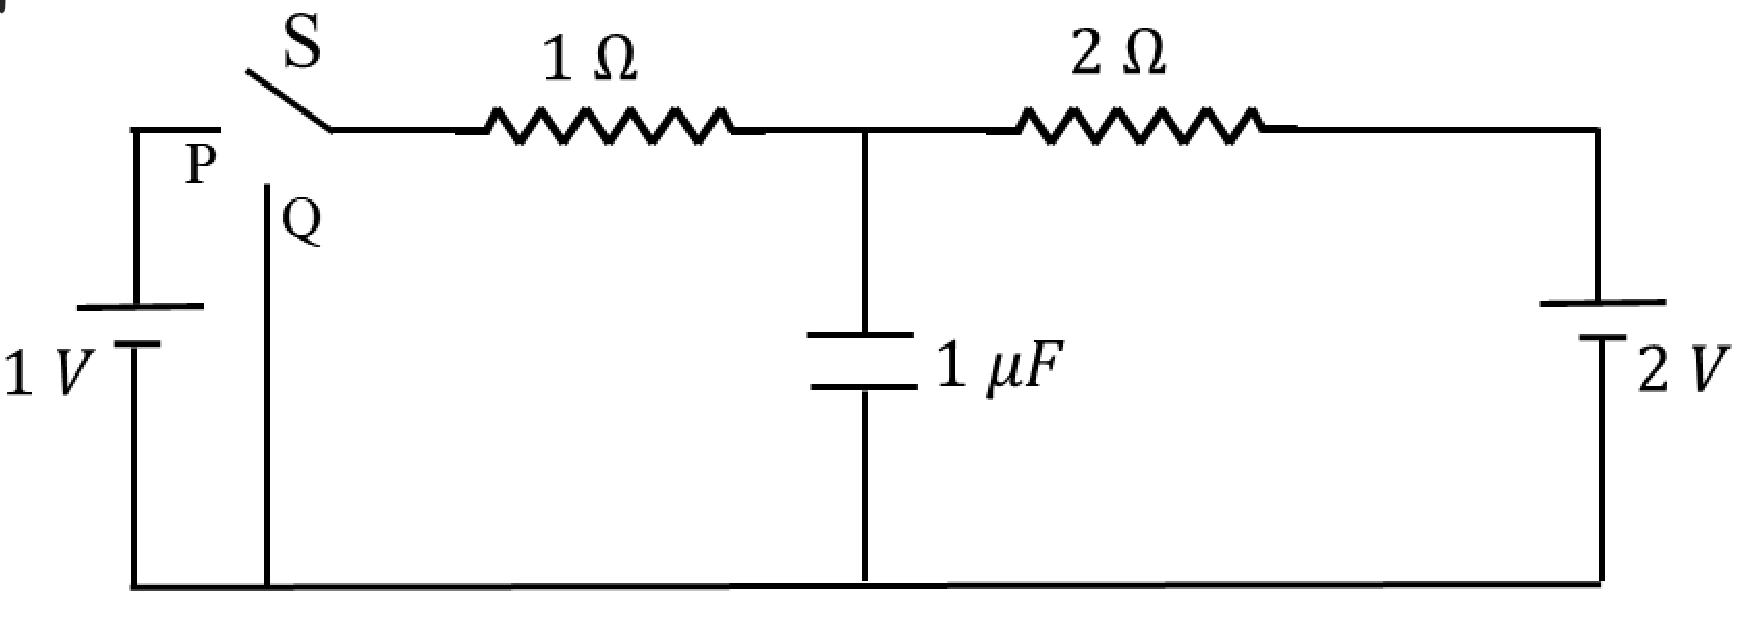
\includegraphics[width=\columnwidth]{figs/ckt.jpg}
			\caption{}
			\label{fig:ckt}
\end{figure}
\item Draw the circuit using latex-tikz.\\
\solution The following code yields Fig.\ref{fig:qn}
\begin{lstlisting}
wget https://github.com/Pradeep8802/EE3900-Digital-Signal-Processing/blob/main/cktsig/Tikz%20Circuits/2.2.tex
\end{lstlisting}
\begin{figure}[!ht]
 \centering
   \begin{circuitikz}[scale=0.7]
 
	\draw (0,0) to [battery1,l_=$1V$] ++(0,-3)
	
	to ++(11.5,0) to [battery1,l_=$2V$,invert]++(0,3)
	
	to [american resistor,l_=$2\Omega$] ++(-6,0)
	
	to [capacitor,l_=$1 \mu F$] ++(0,-3);
	
	\draw (0,0) to ++(0.7,0) node[anchor=north east]{P};
	
	\draw (1,-3) to ++(0,2.6)node[anchor=north west]{Q};
	
	\draw (4.5,0) to ++(1.5,0);
	
	\draw (4.5,0) to [american resistor,l_=$1\Omega$]++(-2,0) 
	
	to ++(-0.8,0.5)node[anchor=south west]{S};
	
\end{circuitikz}

\caption{Given Circuit}
\label{fig:qn}
\end{figure}

\item Find $q_1$.\\
\solution
Before switching S to Q:
\begin{figure}
 %\centering
   \begin{circuitikz}[scale=0.6]
	\draw (0,0) to [battery1,l_=$1V$,i^>=$i$] ++(0,-3)
	to ++(11.5,0) to [battery1,l_=$2V$,invert,i>^=$i$]++(0,3)
	to [american resistor,l_=$2\Omega$,i^>=$i$] ++(-6,0)
	to [capacitor,l_=$1 \mu F$] ++(0,-3);
	\draw (0,0) to ++(2.5,0);
	\draw (4.5,0) to ++(1.5,0);
	\draw (4.5,0) to [american resistor,l_=$1\Omega$,i>^=$i$]++(-2,0) ;
\end{circuitikz}

\caption{Before switching S to Q}
%\label{fig:c1}
\end{figure}
At steady state, which achieved when switch S is at P for long time capacoitor behaves as an open switch, hence current through capacitor is $0$,
Let $i$ be the current flowing in the circuit at steady state. Applying KVL ,
\begin{align}
1-i-2i-2=0\\
3i=-1 \Rightarrow i=\frac{-1}{3}A
\end{align}
Potential Difference across the capacitor at steady state is
\begin{align}
1-\brak{\frac{-1}{3}}=\frac{4}{3}V\\
q_1=\frac{4}{3} \cdot 1\\
=\frac{4}{3} \mu C
\end{align}
	\item Show that the Laplace transform of $u(t)$ is $\frac{1}{s}$ and find the ROC.\\
	\solution We know that Laplace Transform fo function $f(t)$ is given as $F(s)$,
	\begin{align}
		\label{eq:LaplaceTrans}
	F(s)&= \int_{0}^{\infty} f(t)e^{-st} \,dt \\
\end{align}
For $u(t)$, we have,
\begin{align}
	F(s)&=\int_{0}^{\infty} u(t)e^{-st} \,dt
\end{align}
	Using \eqref{eq:unit-step},
	\begin{align}
	F(s)&=\int_{0}^{\infty} u(t)e^{-st} \,dt\\
	&=\int_{0}^{\infty} e^{-st} \,dt\\
	&=-\brak{0-\frac{1}{s}}\\
	&=\frac{1}{s}
	\end{align}
	ROC is $ Re(s)>0$ since for $s>0$, $e^{-st}<\infty$ for $t \to \infty$
	\begin{figure}[!ht]
			\centering
			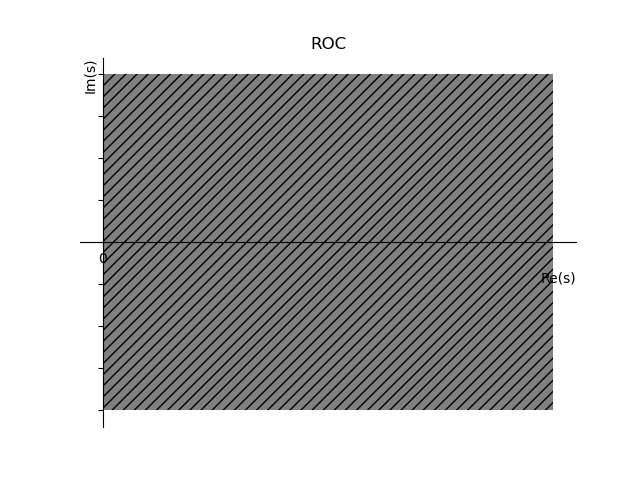
\includegraphics[width=\columnwidth]{figs/2.4}
			\caption{}
			\label{fig:roc1}
\end{figure}
	\item Show that 
		\begin{align}
			e^{-at}u(t) \system{L} \frac{1}{s+a}, \quad a > 0
		\end{align}
		and find the ROC.\\
		\solution From \ref{eq:LaplaceTrans},
		\begin{align}
		F(s)&=\int_{0}^{\infty} u(t)e^{-at}e^{-st} \,dt\\
		&=\int_{0}^{\infty} u(t)e^{-\brak{s+a}t} \,dt\\
		&=\int_{0}^{\infty} e^{-\brak{s+a}t} \,dt\\
		&=-\brak{0-\frac{1}{s+a}}\\
		&=\frac{1}{s+a}
		\end{align}
		ROC is
		\begin{align}
		Re(s)+a>0 \Rightarrow  Re(s)>-a
		\end{align}
		\begin{figure}[!ht]
			\centering
			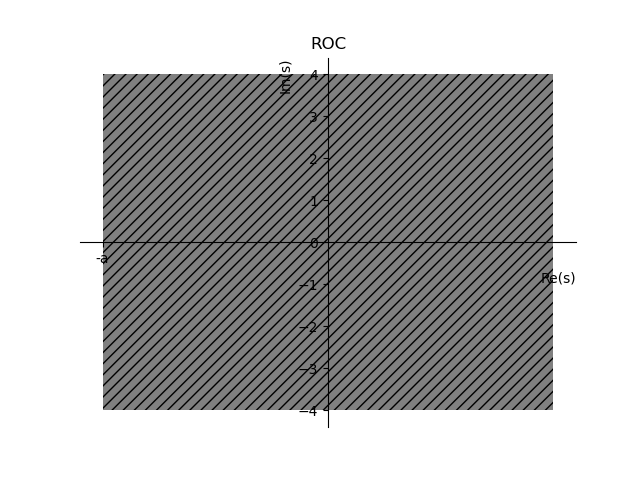
\includegraphics[width=\columnwidth]{figs/2.5.png}
			\caption{}
			\label{fig:roc2}
\end{figure}
	\item Now consider the following resistive circuit transformed from 
			Fig. \ref{fig:ckt}
		\begin{figure}[!ht]
			\centering
			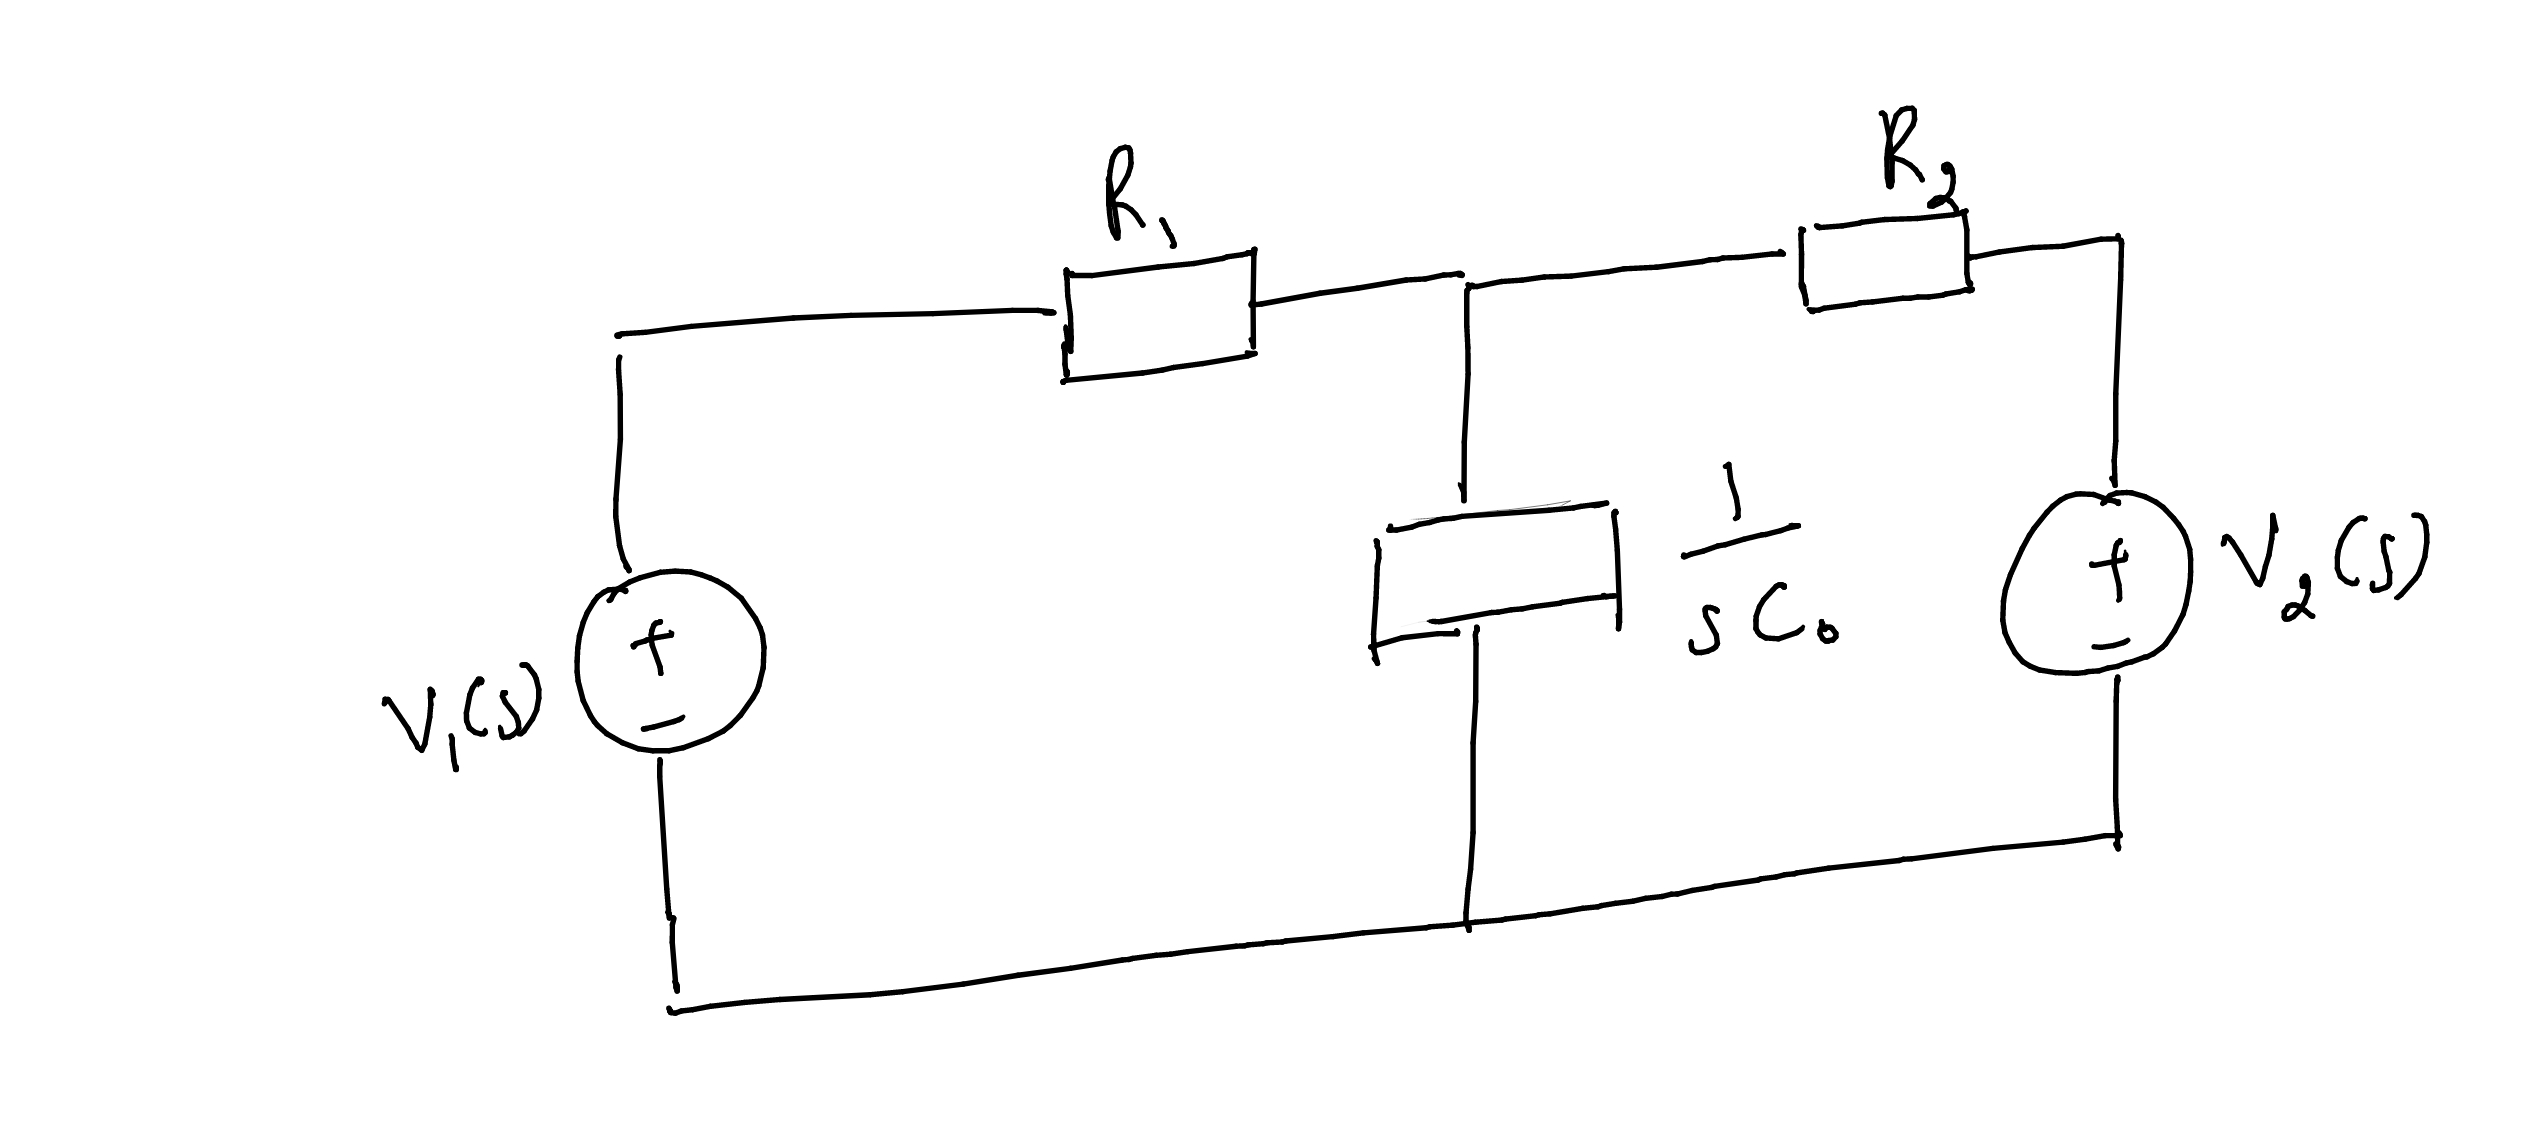
\includegraphics[width=\columnwidth]{figs/lap-ckt.jpg}
			\caption{}
			\label{fig:lap-ckt}
\end{figure}
		where 
		\begin{align}
			u(t) \system{L} V_1(s)
			\\
			2u(t) \system{L} V_2(s)
		\end{align}
		Find the voltage across the capacitor $V_{C_0}(s)$.\\
		\solution
		\begin{align}
		R_{eff}=\frac{1}{1+\frac{1}{2}}
		=\frac{2}{3} \Omega\\
		V_{eff}=\frac{1}{1+\frac{1}{2}}
		=\frac{2}{3}V
		\end{align}
		%Effective Circuit in Laplacian Space is
\begin{align}
V_{C_0}(s)&=V_{S}(s)\frac{C_{0}}{C_{0}+R_{eff}}\\
&=\brak{\frac{4}{3s}}\brak{\frac{\frac{1}{s}}{\frac{1}{s}+\frac{2}{3}}}\\
\label{eq:laptr}
&=\frac{3+4s}{3s\brak{s+\frac{3}{2}}}
\end{align}
	\item Find $v_{C_0}(t)$.  Plot using python.\\
	\solution Running the following code gives the plot.
	\begin{lstlisting}
		wget https://github.com/Pradeep8802/EE3900-Digital-Signal-Processing/tree/main/cktsig/codes/2.7.py
	\end{lstlisting}
	
	Using \eqref{eq:laptr},
	\begin{align}
	\frac{3+4s}{3s\brak{s+\frac{3}{2}}}&=\frac{2}{3s}+\frac{2}{3(\frac{3}{2}+s)}
	\end{align}
	Apply inverse Laplacian Transform,
	\begin{align}
	V_{C_0}(s)\system{L^{-1}}V_{C_0}(t)\\
	\laplaceinv{V_{C_0}(s)}&=\laplaceinv{\frac{2}{3s}+\frac{2}{3(\frac{3}{2}+s)}}\\
&=	\laplaceinv{\frac{2}{3s}}-\frac{2}{3}\laplaceinv{\frac{1}{\frac{3}{2}+s}}
\end{align}
Since,
\begin{align}
\laplaceinv{\frac1s}&=u(t)\\
\laplaceinv{\frac{1}{s-a}}&=e^{at}u(t)
\end{align}
Using the above equations,
\begin{align}
V_{C_0}(t)=\frac{2}{3}\brak{ 1+e^{\frac{-3}{2} t}}u(t)
	\end{align}
	\begin{figure}[!ht]
			\centering
			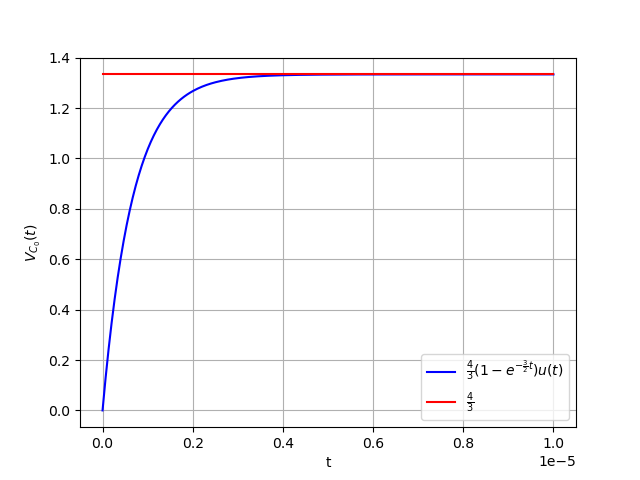
\includegraphics[width=\columnwidth]{figs/2.7.png}
			\caption{Plot of $V_{C_0}(t)$}
			\label{fig:lap}
\end{figure}
	\item Verify your result using ngspice.\\
\solution \begin{figure}[!ht]
			\centering
			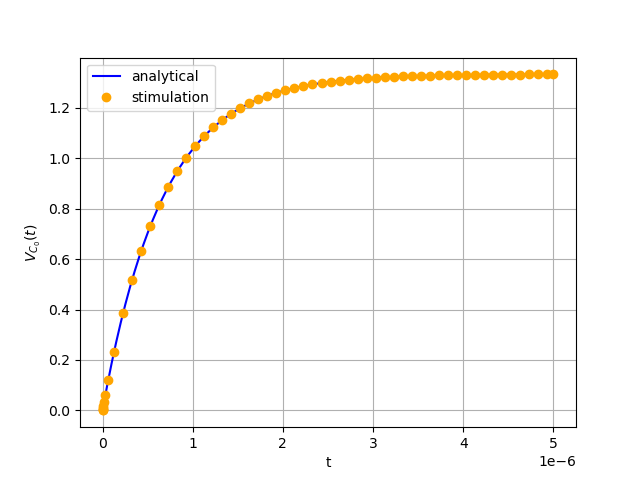
\includegraphics[width=\columnwidth]{figs/2.8.png}
			\caption{}
			\label{fig:ngspice}
\end{figure}

\item Obtain Fig. \ref{fig:lap} using the equivalent differential equation

\solution Results obtained can be verified by running the following code.
\begin{lstlisting}
	wget https://github.com/Pradeep8802/EE3900-Digital-Signal-Processing/tree/main/cktsig/codes/2.8.cir
\end{lstlisting}
And is plotted using the below code.
\begin{lstlisting}
	wget https://github.com/Pradeep8802/EE3900-Digital-Signal-Processing/tree/main/cktsig/codes/2.8.py
\end{lstlisting}
Using Kirchoff's junction law
\begin{align}
	\frac{v_c(t) - v_1(t)}{R_1} + \frac{v_c(t) - v_2(t)}{R_2} + \frac{\der{q}}{\der{t}} = 0
\end{align}
where $q(t)$ is the charge on the capacitor

On taking the Laplace transform on both sides of this equation
\begin{align}
	\frac{V_c(s) - V_1(s)}{R_1} + \frac{V_c(s) - V_2(s)}{R_2} + \brak{sQ(s) - q(0^-)} = 0
\end{align}

But $q(0^-) = 0$ and 
\begin{align}
	q(t) &= C_0v_c(t) \\
	\implies Q(s) &= C_0V_c(s)
\end{align}

Thus
\begin{align}
	&\frac{V_c(s) - V_1(s)}{R_1} + \frac{V_c(s) - V_2(s)}{R_2} + sC_0V_c(s) = 0 \\
	\implies &\frac{V_c(s) - V_1(s)}{R_1} + 	\frac{V_c(s) - V_2(s)}{R_2} + \frac{V_c(s) - 0}{\frac{1}{sC_0}} = 0 
\end{align}

which is the same equation as the one we obtained from Fig. \ref{fig:lap}

\end{enumerate}

 \section{Initial Conditions}
\begin{enumerate}[label=\arabic*.,ref=\thesection.\theenumi]
\numberwithin{equation}{section}
\item Find $q_2$ in Fig. \ref{fig:ckt}.\\
			\solution At steady state capacitor behaves as an open switch. Hence $V_{C_0}=V_{1 \Omega}$.\\
			Let $i$ be the current in the circuit. Using KVL,
			\begin{align}
				2-2i-i=0 \implies i=\frac{2}{3}\\
				V_{1 \Omega}=i \times 1= \frac{2}{3} V\\
			V_{C_0}=\frac{q_2}{C_0}=V_{1 \Omega}=\frac{2}{3}\\
			\implies q_2=\frac{2}{3} \mu C
			\end{align}
\item Draw the equivalent $s$-domain resistive circuit when S is switched to position Q.  Use variables $R_1, R_2, C_0$ for the passive elements.
Use latex-tikz.
		\label{prob:init}
		\\\solution 
	\begin{figure}[!ht]
 \centering
 \begin{circuitikz}[scale=1.5]
  \draw (0,0) to [generic,l=$R_1$]++(2,0) to[generic,l=$R_2$]++(2,0)
  to [battery1,l=$\frac2s V$]++(0,-2) to ++(-2,0)
  to [generic,l=$\frac{1}{sC_0}$]++(0,1) to [battery1,l=$\frac{4}{3s}V$,invert]++(0,1);
  \draw (0,0) to ++(0,-2) to ++(2,0);
  \end{circuitikz}

\caption{After switching S to Q}
\label{fig:sq}
\end{figure}
		\item $V_{C_0}(s)$ = ? \\
		\solution Let voltage across capacitor be $V$. Using KCL at node in Fig. \ref{fig:sq}
\begin{align}
    \frac{V - 0}{R_1} + \frac{V - \frac{2}{s}}{R_2} + sC_0\brak{V - \frac{4}{3s}} = 0 \\
\implies V_{C_0}(s) = \frac{\frac{2}{sR_2} + \frac{4C_0}{3}}{\frac{1}{R_1} + \frac{2}{R_2} + sC_0}
\label{eq:v2-s}
\end{align} 
	\item $v_{C_0}(t)$ = ? Plot using python.\\
	\solution Running the following code gives the plot.
	\begin{lstlisting}
		wget https://github.com/Pradeep8802/EE3900-Digital-Signal-Processing/tree/main/cktsig/codes/3.4.py
	\end{lstlisting}
	From \eqref{eq:v2-s},
\begin{align}
    &V_{C_0}(s) = \frac{4}{3}\brak{\frac{1}{\frac{1}{C_0}\brak{\frac{1}{R_1} + \frac{1}{R_2}}+s}} \nonumber \\
    &+ \frac{2}{R_2\brak{\frac{1}{R_1} +\frac{1}{R_2}}}\brak{\frac{1}{s} - \frac{1}{\frac{1}{C_0}\brak{\frac{1}{R_1} + \frac{1}{R_2}} + s}}
\end{align}
Taking an inverse Laplace Transform,
\begin{align}
    &v_{C_0}(t) = \frac{4}{3}e^{-\brak{\frac{1}{R_1} + \frac{1}{R_2}}\frac{t}{C_0}}u(t) \nonumber \\ 
    &+ \frac{2}{R_2\brak{\frac{1}{R_1}+\frac{1}{R_2}}}\brak{1 - e^{-\brak{\frac{1}{R_1} + \frac{1}{R_2}}\frac{t}{C_0}}}u(t)
\end{align}
Substituting values gives
\begin{align}
    v_{C_0}(t) = \frac{2}{3}\brak{1 +e^{-\brak{1.5 \times 10^6}t}}u(t)
    \label{eq:v2-t}
\end{align}
\begin{figure}[!ht]
			\centering
			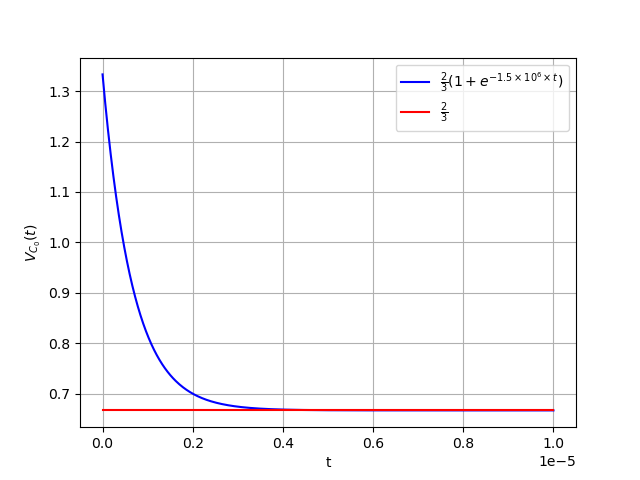
\includegraphics[width=\columnwidth]{figs/3.4.png}
			\caption{Plot of $V_{C_0}(t)$}
			%\label{fig:lap-ckt}
\end{figure}
	\begin{figure}[!ht]
	\centering
	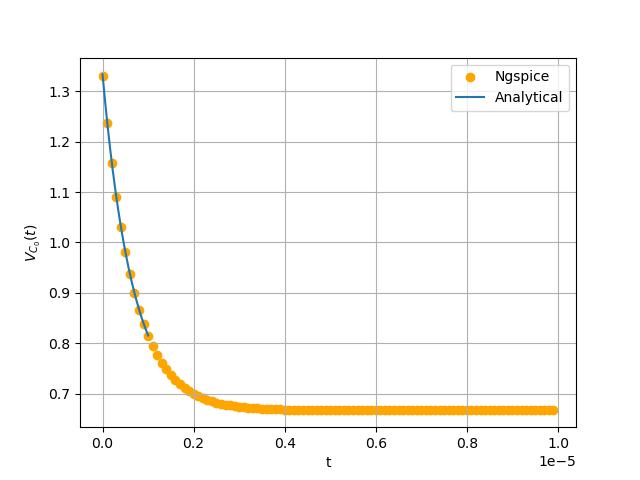
\includegraphics[width=\columnwidth]{figs/3.5.png}
	\caption{ngspice plot of $V_{C_0}(t)$} 
	\label{fig:ngspice2}
\end{figure}
	\item Verify your result using ngspice.\\
	\solution Results obtained can be verified by running the following code.
	\begin{lstlisting}
wget https://github.com/Pradeep8802/EE3900-Digital-Signal-Processing/tree/main/cktsig/codes/3.5.cir
	\end{lstlisting}
Runningn the below code plots the figure \ref{fig:ngspice2}, and verifies our result.
	\begin{lstlisting}
wget https://github.com/Pradeep8802/EE3900-Digital-Signal-Processing/tree/main/cktsig/codes/3.5.py
	\end{lstlisting}



	\item Find $v_{C_0}(0-), v_{C_0}(0+)$ and  $v_{C_0}(\infty) $.\\
\solution From the initial conditions,
\begin{align}
    v_{C_0}(0-) = \frac{q_1}{C} = {\frac{4}{3}}{V}
\end{align}
Using \eqref{eq:v2-t},
\begin{align}
    v_{C_0}(0+) &= \lim_{t \to 0+}v_{C_0}(t) = {\frac{4}{3}}{V} \\
    v_{C_0}(\infty) &= \lim_{t \to \infty}v_{C_0}(t) = {\frac{2}{3}}{V}
\end{align}

\item Obtain Fig. \ref{prob:init} using the equivalent differential equation

\solution Using Kirchoff's junction law
\begin{align}
	\label{eq:a}
	\frac{v_c(t) - 0}{R_1} + \frac{v_c(t) - v_2(t)}{R_2} + \frac{\der{q}}{\der{t}} = 0
\end{align}
where $q(t)$ is the charge on the capacitor.
On taking the Laplace transform on both sides of the equation \eqref{eq:a}, we get,
\begin{align}
	\frac{V_c(s) - 0}{R_1} + \frac{V_c(s) - V_2(s)}{R_2} +sQ(s) - q(0^-) = 0
\end{align}

But $q(0^-) = \frac43 C_0$ and 
\begin{align}
	q(t) &= C_0v_c(t) \\
	\implies Q(s) &= C_0V_c(s)
\end{align}

Thus
\begin{align}
	&\frac{V_c(s) - 0}{R_1} + \frac{V_c(s) - V_2(s)}{R_2} + \brak{sC_0V_c(s) - \frac43 C_0} = 0 \\
	\implies &\frac{V_c(s) - 0}{R_1} + 	\frac{V_c(s) - V_2(s)}{R_2} + \frac{V_c(s) - \frac{4}{3s}}{\frac{1}{sC_0}} = 0 
\end{align}

which is the same equation as the one we obtained from Fig. \ref{prob:init}
\end{enumerate}
	

\section{Bilinear Transform}
\begin{enumerate}[label=\thesection.\arabic*.,ref=\thesection.\theenumi]
	\item In Fig. \ref{fig:ckt}, consider the case when $S$ is switched to $Q$ right in the beginning. Formulate the differential equation
	
	\solution 
		\begin{figure}[!ht]
		\centering
		 \begin{circuitikz}[scale=0.7]
	\draw (0,0) to (0,-3)
	to ++(11.5,0) to [battery1,l_=$2V$,invert]++(0,3)
	to [american resistor,l_=$2\Omega$] ++(-6,0)
	to [capacitor,l_=$1 \mu F$] ++(0,-3);
	\draw (0,0) to ++(2.5,0);
	\draw (4.5,0) to ++(1.5,0);
	\draw (4.5,0) to [american resistor,l_=$1\Omega$]++(-2,0) ;
\end{circuitikz}

		\caption{Switch S connected to Q initially}
		\label{fig:4.1}
	\end{figure}
Considering KCL on the circuit \ref{fig:4.1}, we get the differential equuation as 
	\begin{align}
		\label{eq:diff.4.1}
		&\frac{v_c(t) - 0}{R_1} + \frac{v_c(t) - v_2(t)}{R_2} + \frac{\der{q}}{\der{t}} = 0 \\
		\implies &\frac{v_c(t)}{R_1} + \frac{v_c(t) - v_2(t)}{R_2} + C_0\frac{\der{v_c}}{\der{t}} = 0
	\end{align}
Here we have $q(0)=0$, since initially the capacitor is uncharged.
	
	\item Find $H(s)$ considering the ouput voltage at the capacitor
	
	\solution Applying laplace transform to the equation \eqref{eq:diff.4.1}, we get
		\begin{align}
		&\frac{V_c(s)}{R_1} + \frac{V_c(s) - V_2(s)}{R_2} + \mathcal{L}(\frac{\der{q}}{\der{t}})= 0 \\
		&\frac{V_c(s)}{R_1} + \frac{V_c(s) - V_2(s)}{R_2} + sQ(s) - q(0) = 0 \\
		&\frac{V_c(s)}{R_1} + \frac{V_c(s) - V_2(s)}{R_2} + sQ(s) - 0 = 0 \\
		\implies &V_c(s) \brak{\frac{1}{R_1} + \frac{1}{R_2}} + sC_0V_c(s) = \frac{V_2(s)}{R_2} \\
		\implies &\frac{V_c(s)}{V_2(s)} = \frac{\frac{1}{R_2}}{\frac{1}{R_1} + \frac{1}{R_2} + sC_0}
	\end{align}
	Here, $Q(s)$ is the laplace transform of q, $V_c(s)$ is laplace transform of $v_c(t)$.
	Hence, the transform function($H(s)$) is 
	\begin{align}
		H(s) &= \frac{V_c(s)}{V_2(s)} \\
		&=\frac{\frac{1}{R_2C_0}}{s + \frac{1}{R_1C_0} + \frac{1}{R_2C_0}}
	\end{align}
	Substituting values of $R_1=1\Omega$,$R_2=2\Omega$ and $C_0=1\mu F$, we get,
	\begin{align}
		H(s) &= \frac{0.5}{s 10^{-6} + 1.5}\\
		\label{eq:Hs}
		\implies H(s)&=\frac{5 \times 10^5}{s + 1.5 \times 10^6}
	\end{align}

\begin{figure}[!ht]
	\centering
	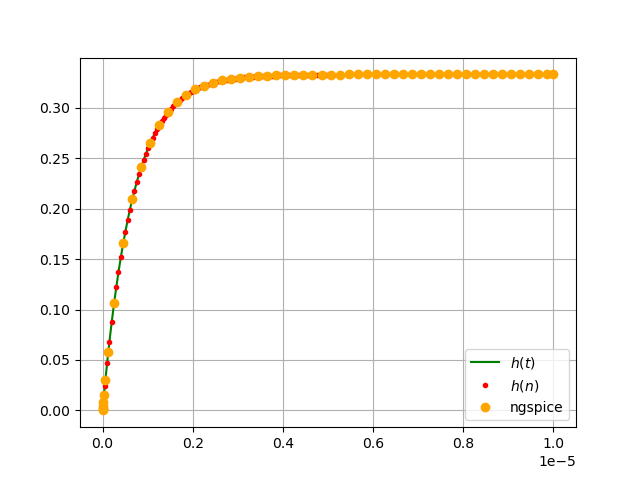
\includegraphics[width=\columnwidth]{./figs/4.2.png}
	\caption{ngspice plot of $H(t)$}
	\label{fig-4.2}
\end{figure}
The following python code plots the figure \ref{fig-4.2}
\begin{lstlisting}
	wget https://github.com/Pradeep8802/EE3900-Digital-Signal-Processing/tree/main/cktsig/codes/4.2.py
\end{lstlisting}
%Applying inverse Laplace transform to equation \eqref{eq:Hs}, we get,
%\begin{align}
%H(t)=5\times 10^{5} e^{-1.5\times 10^{6}}
%H(t)=\frac{1}{3} \frac{(1 - (1 - 7.5 10^5 t )}{(1 + 7.5 10^{5} t)}^{10^{7}n}	
%\end{align}
	\item Plot $H(s)$.  What kind of filter is it?\\
	\solution THe below python code plots the Figure \ref{fig-4.3}
	\begin{lstlisting}
	wget https://github.com/Pradeep8802/EE3900-Digital-Signal-Processing/tree/main/cktsig/codes/4.3.py
	\end{lstlisting}
	\begin{figure}[!ht]
		\centering
		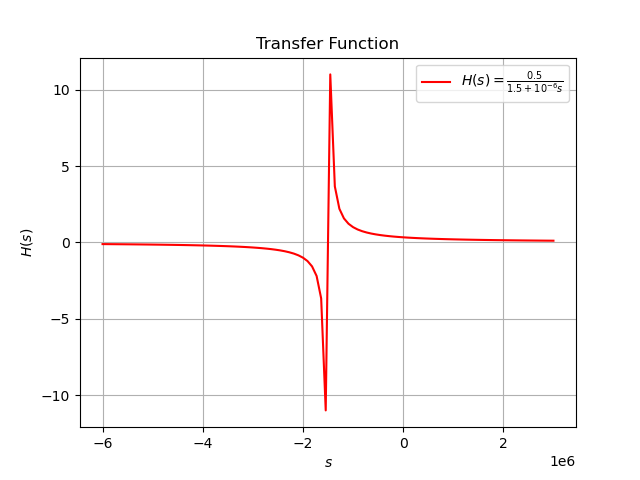
\includegraphics[width=\columnwidth]{./figs/4.3.png}
		\caption{Plot of $H(s)$}
		\label{fig-4.3}	
	\end{figure}
	Considering the frequency-domain transfer function ($H(s=e^{j\omega})$), from \eqref{eq:Hs},we get
	\begin{align}
		\label{eq:Hw}
		H(s=j\omega) &= \frac{5 \times 10^5}{j\omega + 1.5 \times 10^6} \\
		\implies \abs{H(s=j\omega)} &= \frac{5 \times 10^5}{\sqrt{\omega^2 + 2.25\times10^{12}}}
	\end{align}
Clearly from \eqref{eq:Hw}, as $\omega$ increases, $H(s=j\omega)$ decreases(inverse proportionality). When high frequency signals( large values of $\omega$) pass through this transfer function ($H(s=j\omega$)), they become negligible, which results in removing high frequnecy signals and allowing only low frequency signal to pass. Hence, this is a low-pass filter.
	\item Using trapezoidal rule for integration, formulate the difference equation by considering 
	\begin{align}
		y(n) = y(t)\vert_{t=n}
	\end{align}
	\solution
	In the equation \eqref{eq:diff.4.1}, we have
	\begin{align}
		\frac{\der{q}}{\der{t}}&=C_0\frac{\der{v_c}}{\der{t}}\\
		v_2(t)&=2u(n)
	\end{align} 
Hence,
	\begin{align}
		&\frac{v_c(t)}{R_1} + \frac{v_c(t) - v_2(t)}{R_2} + C_0\frac{\der{v_c}}{\der{t}} = 0 \\
		\implies &C_0\frac{\der{v_c}}{\der{t}} = \frac{2u(t)-v_c(t)}{R_2} - \frac{v_c(t)}{R_1} \\
		\implies &\frac{\der{v_c}}{\der{t}} = \frac{2u(t)-v_c(t)}{R_2 C_0} - \frac{v_c(t)}{R_1 C_0} \\
		\label{eq:trap}
		\implies &\left.v_c(t)\right|_{t=n}^{n+1} = \int_{n}^{n+1} \brak{\frac{2u(t)-v_c(t)}{R_2C_0} - \frac{v_c(t)}{R_1C_0}} \der{t}
	\end{align}
	
	From trapezoidal rule of integration
	\begin{align}
		\label{eq:traprule}
		\int_a^b f(t) \der{t} \approx \frac{b-a}{2} (f(a) + f(b))
	\end{align}
	Apply \eqref{eq:traprule}, to the RHS of the equation \eqref{eq:trap}, we get,
	\begin{align}
		\int_{n}^{n+1} \frac{2u(t)-v_c(t)}{R_2C_0} &- \frac{v_c(t)}{R_1C_0} \der{t}=\frac{1}{R_2C_0}\brak{u(n)+u(n+1)}\\&- \frac12(y(n+1) + y(n))\brak{\frac{1}{R_1C_0} + \frac{1}{R_2C_0}}
	\end{align}
	Considering $y(t) = v_c(t)$, from \eqref{eq:trap}, we get,
	\begin{multline}
		y(n+1) - y(n) = \frac{1}{R_2C_0}\brak{u(n)+u(n+1)} \\
		- \frac12(y(n+1) + y(n))\brak{\frac{1}{R_1C_0} + \frac{1}{R_2C_0}}
	\end{multline}
	Thus, the difference equation is
	\begin{multline}
		\implies y(n+1) \brak{1 + \frac{1}{2R_1C_0} + \frac{1}{2R_2C_0}} \\= y(n) \brak{1 - \frac{1}{2R_1C_0} - \frac{1}{2R_2C_0}} \\+ \frac{1}{R_2C_0}\brak{u(n)+u(n+1)}
	\end{multline}
	
	\item Find $H(z)$\\
	
	\solution Let $\z{y(n)} = Y(z)$
	
	On taking $\mathcal{Z}$-transform on both sides of the difference equation, we get,
	\begin{multline}
		zY(z)\brak{1 + \frac{1}{2R_1C_0} + \frac{1}{2R_2C_0}} \\= Y(z)\brak{1 - \frac{1}{2R_1C_0} - \frac{1}{2R_2C_0}} \\+ \frac{1}{R_2C_0} \brak{\frac{1}{1-z^{-1}} + \frac{z}{1-z^{-1}}}
	\end{multline}
	\begin{multline}
		Y(z)\brak{z + \frac{z}{2R_1C_0} + \frac{z}{2R_2C_0} - 1 + \frac{1}{2R_1C_0} + \frac{1}{2R_2C_0}} \\
		= \frac{1}{R_2C_0} \frac{1+z}{1-z^{-1}}
	\end{multline}
	Here, since $v_2(t) = 2 \forall t \ge 0\\$ \\
	Initial voltage is given as,
	\begin{align}
		\implies x(n) &= 2u(n) \\
		\implies X(z) &= \frac{2}{1-z^{-1}} &&\abs{z} > 1
	\end{align}
	Thus, the transfer function in $z$-domain is
	\begin{align}
		H(z) &= \frac{Y(z)}{X(z)} \\
		&= \frac{\frac{1+z}{2R_2C_0}}{z + \frac{z}{2R_1C_0} + \frac{z}{2R_2C_0} - 1 + \frac{1}{2R_1C_0} + \frac{1}{2R_2C_0}} \\
		&= \frac{\frac{1 + z^{-1}}{2R_2C_0}}{1 + \frac{1}{2R_1C_0} + \frac{1}{2R_2C_0} - z^{-1} + \frac{z^{-1}}{2R_1C_0} + \frac{z^{-1}}{2R_2C_0}}
	\end{align}
	Substituting the values of $R_1$,$R_2$ and $C_0$, we get,
	\begin{align}
		\label{eq:4.5}
		H(z) &= \frac{2.5\times10^5 (1+z^{-1})}{7.5\times10^5 + 1 + (7.5\times10^5 - 1)z^{-1}}
	\end{align}
Where, ROC of $H(z)$ is,
	\begin{align}
		\abs{z} &> 1 \cap \abs{z}>\abs{\frac{7.5\times10^5 - 1}{7.5\times10^5 + 1}} \\
		\implies \abs{z} &> 1
	\end{align}

	\item How can you obtain $H(z)$ from $H(s)$?
	
	\solution The $Z$-transform can be obtained from the Laplace transform by the substitution
	\begin{align}
		s &= \frac{2}{T} \frac{1-z^{-1}}{1+z^{-1}}
	\end{align}
	where $T$ is the sampling time period, used in the trapezoidal rule. Here, its value is $1$. This known as the bilinear transform.\\
	From \eqref{eq:trap}, we have,
	\begin{align}
		H(z) &= \frac{\frac{1}{R_2C_0}}{2\frac{1-z^{-1}}{1+z^{-1}} + \frac{1}{R_1C_0} + \frac{1}{R_2C_0}} \\
		&= \frac{\frac{1 + z^{-1}}{2R_2C_0}}{1-z^{-1}	 + \brak{\frac{1}{2R_1C_0} + \frac{1}{2R_2C_0}}(1 + z^{-1})} \\
		&= \frac{\frac{1 + z^{-1}}{2R_2C_0}}{1 + \frac{1}{2R_1C_0} + \frac{1}{2R_2C_0} - z^{-1} + \frac{z^{-1}}{2R_1C_0} + \frac{z^{-1}}{2R_2C_0}} \\
		\label{eq:4.6}
		&= \frac{2.5\times10^5 (1+z^{-1})}{7.5\times10^5 + 1 + (7.5\times10^5 - 1)z^{-1}}
	\end{align}
Here, this result obtained in the equation \eqref{eq:4.6} is same as the result we obtained in \eqref{eq:4.5}

\item Find $y(n)$ from $H(z)$ and verify whether $y(n) = y(t)|_{t=n}$\\
\solution 
We know that, 
\begin{align}
	Y(z) &= H(z)X(z) \\
	&= \brak{\frac{2.5\times10^5 (1+z^{-1})}{7.5\times10^5 + 1 + (7.5\times10^5 - 1)z^{-1}}} \frac{2}{1-z^{-1}} \\
	\label{eq:4.7}
	&= \frac{\frac{2}{3}}{1-z^{-1}} -\frac{\frac{2}{3}}{7.5\times10^5 + 1 + (7.5\times10^5 - 1)z^{-1}}
\end{align}
Let ROC be $\abs{z}>1$, we know that,
\begin{align}
	\frac{1}{1-z^{-1}} &\system{Z} u(n)\\
	\frac{1}{1-a z^{-1}} &\system{Z} a^{n} u(n)
\end{align}
Applying inverse $\mathcal{Z}$ to the equation \eqref{eq:4.7}, we get 
\begin{align}
	y(n) &= \frac{2}{3}u(n) - \frac{2}{3}\frac{1}{7.5\times10^5 + 1}\brak{-\frac{7.5\times10^5 - 1}{7.5\times10^5 + 1}}^nu(n) \\
\label{eq:4.7.1}
	&= \frac{2}{3} \brak{1 - \frac{(1-7.5\times10^5)^n}{(1+7.5\times10^5)^{n+1}}}u(n)
\end{align}
%If we are sampling the signal at intervals of $T \ll 10^{-5}$, say $\SI[parse-numbers=false]{10^{-7}}{\second}$, i.e., $n = 10^{-7}, 2\times10^{-7},\ldots$
Applying binomial theorem to the equation \eqref{eq:4.7.1}, ($(1+x)^{n} \approx 1+nx$ for $x \ll 1$), we get,
\begin{align}
	\label{eq:4.7.3}
	y(n) &\approx \frac{2}{3} \brak{1 - \frac{1-7.5\times10^5n}{1+7.5\times10^5n}}u(n)
\end{align}
Now, consider $Y(s)$, 
\begin{align}
	Y(s) &= H(s)X(s) \\
	&= \frac{5\times10^5}{s+1.5\times10^6} \frac{2}{s} \\
	\label{eq:4.7.2}
	&= \frac{10^6}{1.5\times10^6} \brak{\frac{1}{s} - \frac{1}{s+1.5\times10^6}}
\end{align}
We know that ,
Let ROC be $\abs{z}>1$, we know that,
\begin{align}
	\frac{1}{s} &\system{L} 1 \quad  \Re(s)>0\\
	\frac{1}{s+a} &\system{L} e^{-at} \quad \Re(s)>-a
\end{align}
Consider ROC as $\Re(s)>0$, applying inverse laplace transform to the equation \eqref{eq:4.7.2}, we get,  
\begin{align}
	y(t) = \frac{2}{3}\brak{1 - e^{-1.5\times10^6t}}u(t)
\end{align}
But for $t \ll 10^-6$, we have
\begin{align}
	e^{-1.5\times 10^6 t} &= \frac{e^{-0.75 \times 10^6 t}}{e^{0.75 \times 10^6 t}} \\
	&\approx \frac{1-7.5\times10^5t}{1+7.5\times10^5t}  
\end{align}
Therefore
\begin{align}
	\label{eq:4.7.4}
	y(t) &\approx \frac{2}{3} \brak{1 - \frac{1-7.5\times10^5t}{1+7.5\times10^5t}} u(t) 
\end{align}
From equations \eqref{eq:4.7.3} and \eqref{eq:4.7.4}, we have,
\begin{align}
	\therefore y(n) &= y(t)|_{t=n}
\end{align}
Hence verified.
\begin{figure}[!ht]
	\centering
	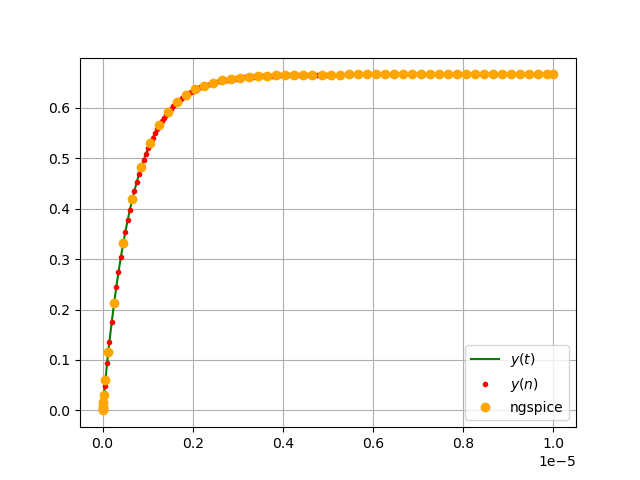
\includegraphics[width=\columnwidth]{./figs/4.7.png}
	\caption{Plot of $y(t)$,$y(n)$ and ngspice}
	\label{fig:4.7}	
\end{figure}
The following python plots the graph \ref{fig:4.7} of $V_C(t)$.
\begin{lstlisting}
wget https://github.com/Pradeep8802/EE3900-Digital-Signal-Processing/tree/main/cktsig/codes/4.7.py
\end{lstlisting}

\end{enumerate}

\end{document}
